%\paragraph{Scene description}
    We run DE algorithm to obtain optimal polices and solution path of our
    optimal control problem in \Cref{eqn:lockdown_vaccination_ocp}. We simulate
    an outbreak with initial conditions according with
    \Cref{fig:initialcondition}, that is, with positive prevalence of all
    epidemiological classes and with parameters enclosed in
    \Cref{tbl:parameters_values}.
    %
    \Cref{fig:lockdowncontrolsignal,fig:vaccinationcontrolsignal} display the
    piecewise optimal control signals that modulate the parameters of lockdown
    release rate $\delta_L$ and vaccination rate $\lambda_V$. Here each signal
    is constant in sub intervals of \SI{4}{days}. We
    display the effect of applied the optimal control
    signal modulation lockdown release in \Cref{fig:lockdowneffect}.
    Upper panel of this figure denotes the optimal release lockdown policy,
    that is the fraction of lockdown individuals that has to release each for
    days. Because initial fraction of individuals under lockdown is around
    \SI{25}{\percent} we observe a exponential output form. Thus middle panel
    display an optimal lockdown in path (in orange) that is under the regarding
    random policy (in blue). This behavior is confirmed the bottom panel, here
    can observe that the susceptible population fraction is above of the random
    controlled and without modulation.
\begin{figure*}
    \centering
    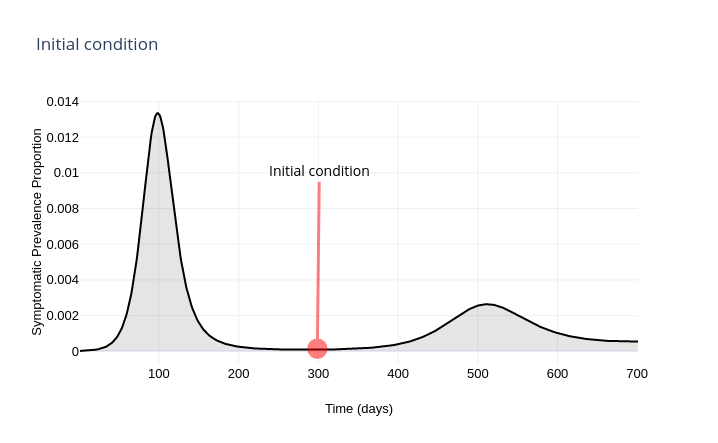
\includegraphics[scale=0.5, keepaspectratio]{figs/InitialCondition}
    \caption[Initial condition]{
        Initial condition scheme. We assume a positive
        prevelance. Forreference, at the date of write this manuscript,
        prevalence in CDMX is
        around \SI{16000}{cases}, see
        \href{https://plotly.com/~sauld/36/}{https://plotly.com/~sauld/36/}
        to display a electronic viewer.}
        \label{fig:initialcondition}
\end{figure*}
%
\begin{figure*}[tbh]
    \centering
    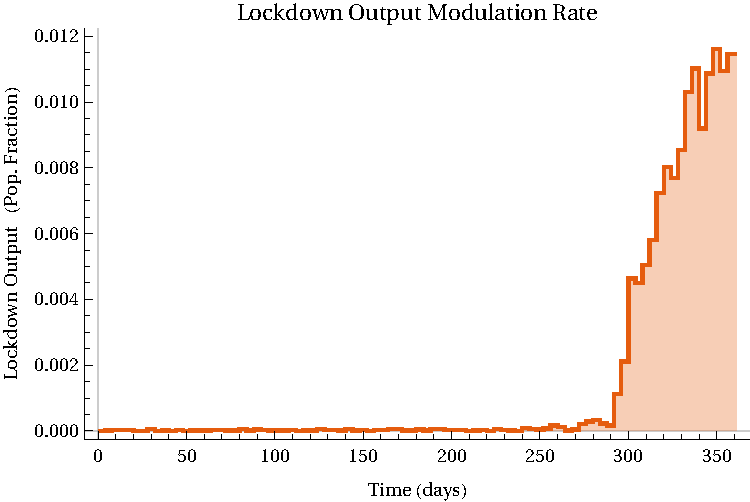
\includegraphics[width=0.7\linewidth]{figs/lockdown_control_signal}
    \caption[Lockdown modulation signal.]{
        Lockdown modulation signal. These piecewise optimal policy suggest
        release more inhabitants under lockdown at
        the final of the outbreak, which is consistent with the prevalence
        curve of reported infected cases.
        \href{https://plotly.com/~AdrianSalcedo/56/}{%
            https://plotly.com/~AdrianSalcedo/56/}
        to display a electronic viewer.
}
    \label{fig:lockdowncontrolsignal}
\end{figure*}

\begin{figure}
    \centering
    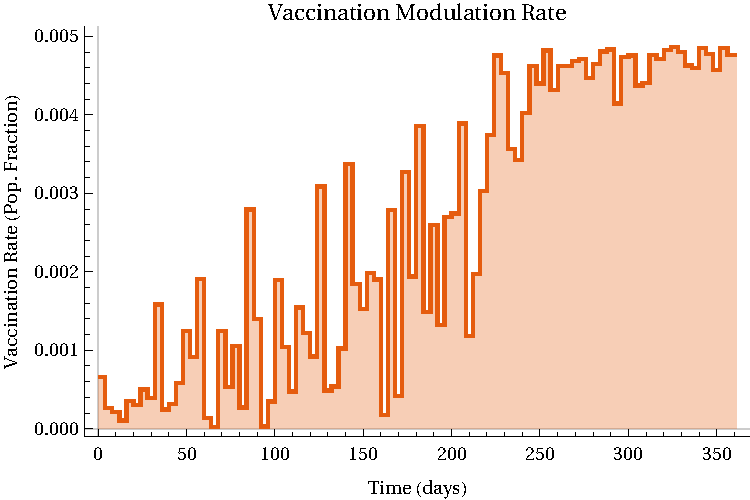
\includegraphics[width=0.7\linewidth]{figs/Vaccination_control_signal}
    \caption[Vaccination rate modulation.]{
        Vaccination rate modulation signal. The optimal policy suggest to
        intensify the vaccination rate at the beginning of outbreak and then
        gradually reduce the vaccination rate intensity.
        \href{https://plotly.com/~AdrianSalcedo/58/}{%
            https://plotly.com/~AdrianSalcedo/58/}
    }
    \label{fig:vaccinationcontrolsignal}
\end{figure}

\begin{figure}[tbh]
    \centering
    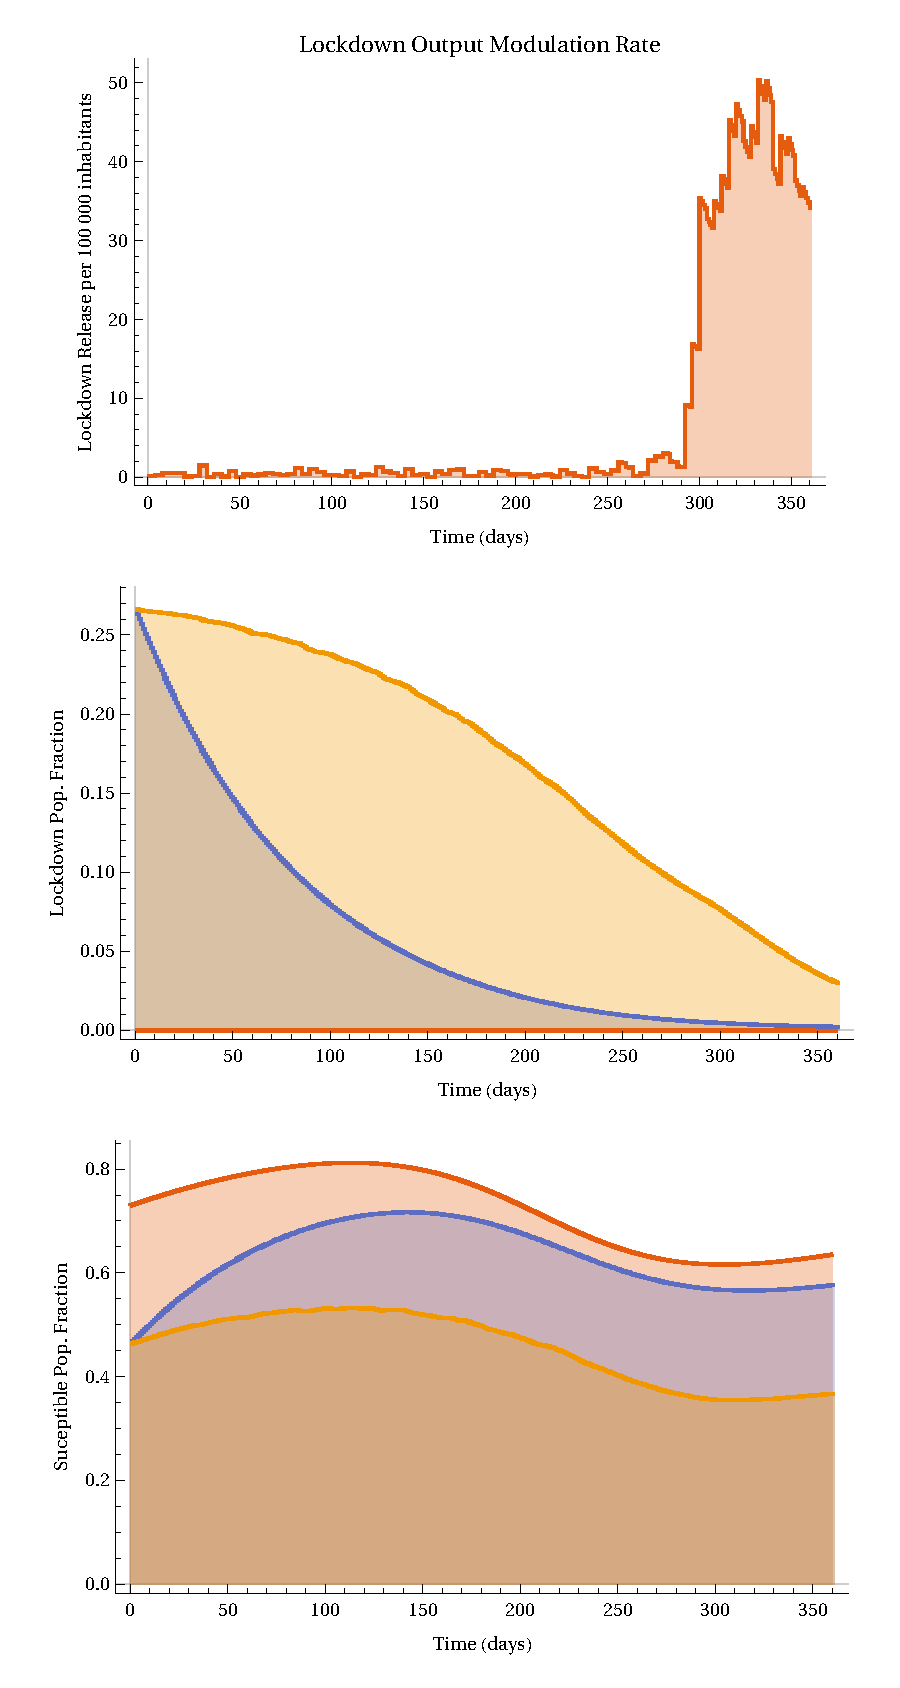
\includegraphics[scale=0.65, keepaspectratio]{figs/LockdownEffect}
    \caption{
        Modulation lock down release.
        (Upper) Optimal release policy defined as the product of the Lockdown
        population $L(t)$ and modulated release rate $(\delta_L + u_L(t))$.
        (Middle) Lockdown likening between the random and optimal controlled
        policies.
        (Bottom) Contrast between the not controlled, random  and optimal
        policy effect in the fraction of susceptible population.
        \href{https://plotly.com/~AdrianSalcedo/60/}{%
            https://plotly.com/~AdrianSalcedo/60/}.
    }
    \label{fig:lockdowneffect}
\end{figure}

\begin{figure*}[tbh]
    \centering
    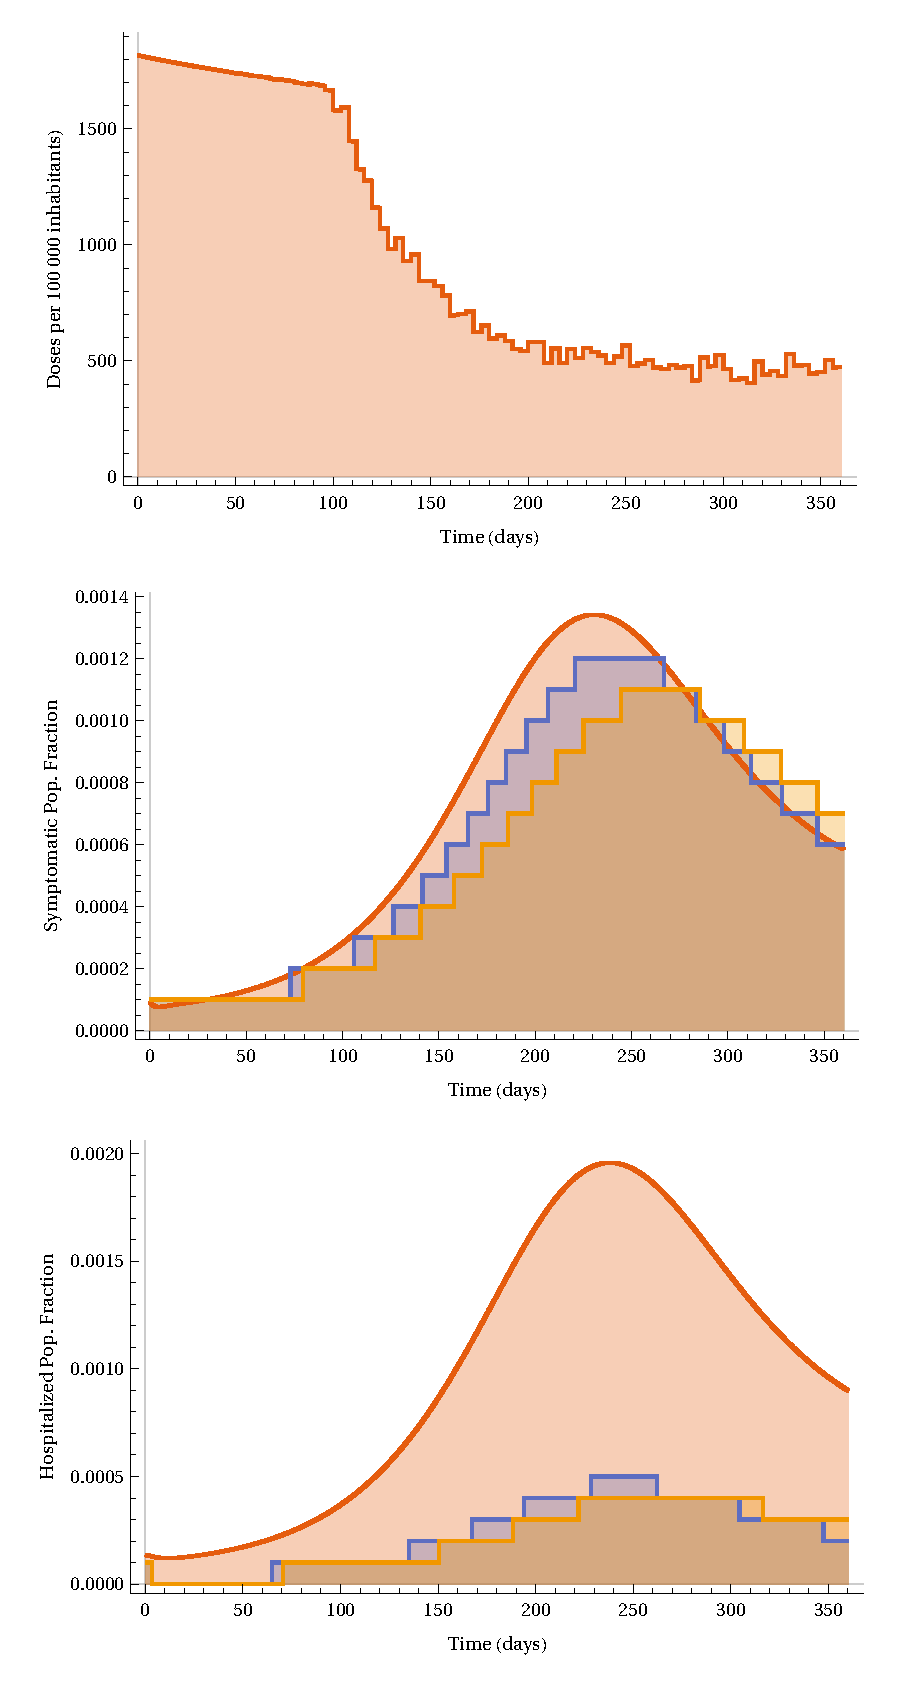
\includegraphics[scale=0.65, keepaspectratio]{figs/VaccinationEffect}
    \caption{
        Effect of the piecewise optimal lockdown-vaccination
        policies in the symptomatic and hospitalized population fraction.
        (Upper) Vaccination doses per day corresponding to the optimal policy.
        (Middle) The effect of lockdown-vaccination intervention in the
        mitigation of prevalence of symptomatic cases. Red solid line
        corresponds to the dynamics without interventions. Blue solid lines is
        the random intervention from a generation of the Differential evolution
        and orange is the regarding optimal policy.
        (Bottom) The effect of the intervention policies in the Hospitalization
        prevalence.
        \href{https://plotly.com/~AdrianSalcedo/61/}{%
        https://plotly.com/~AdrianSalcedo/61/}
    }
    \label{fig:vaccinationeffect}
\end{figure*}
\begin{figure}
    \centering
    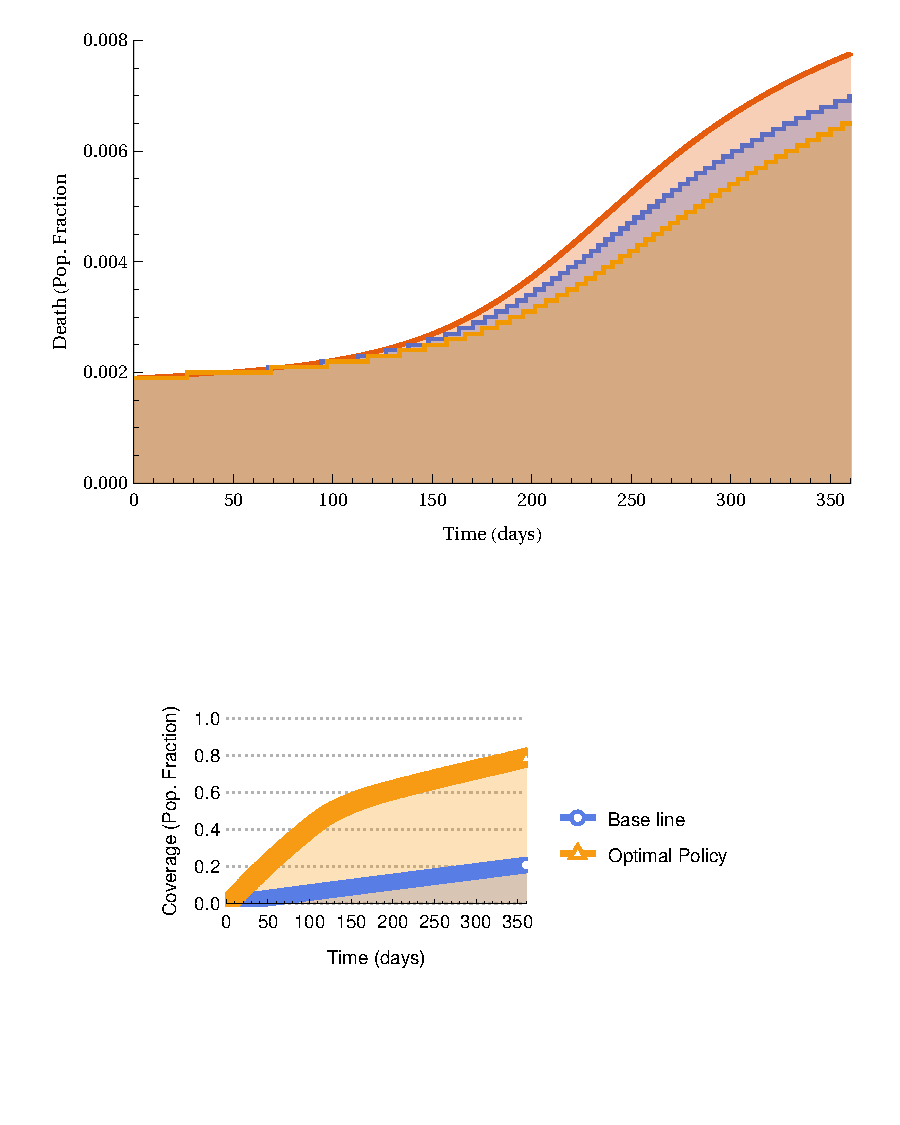
\includegraphics[width=0.7\linewidth]{figs/deathsVaccinationCoverage}
    \caption{Death population fraction and vaccination coverage.
    (Upper) Contra-factual scenario between the incidence of deaths according to
    no intervention, random and optimal lockdown-vaccination policies.
    (Bottom) Likening between vaccination coverage with a minimal base
    vaccination rate and the optimal policy. Here the base vaccination rate
    corresponds to a coverage of \SI{20}{\percent} in two years.
}
    \label{fig:deathsvaccinationcoverage}
\end{figure}

\begin{rmk}
    We define optimal lockdown release policy as the product
    $$[\delta_L + u_L(t)] L,$$ and the vaccine application dose as
    $$
        [\lambda_V + u_V(t)] (L+S+E+I_A+R).
    $$
\end{rmk}

\subsection{Discussion}